% !TEX root = ../thesis-example.tex
%
\chapter{Multiple time series forecasting using ensembles of quasi-randomized functional link neural networks}
\label{sec:rvfl_ensembles}

\section{Introduction}

The goal of ensemble learning is to combine two or more individual statistical/machine learning models - the base models or base learners - into one, in order to obtain an ensemble model, with an improved out-of-sample error over the base models.

\medskip

Ensemble learning is widely used in the winning solutions of machine learning competitions. It allows to achieve very good performances indeed, at the expense of being relatively less interpretable than the base learners. As a consequence, choosing to use ensemble models or a base model for solving a given problem, could sometimes be seen as finding a trade-off between the desire for interpretability and the desire for an highly increased performance. That said, some techniques such as variable importance for ensemble of trees, can give a sense of which predictor contributes the most to the perfomance of the model.

\medskip

In this chapter, we apply three popular ensemble learning methods to multiple time series forecasting: Bootstrap aggregating (cite Efron), known as bagging, Boosting (cite Hothorn et al. (2010), Friedman et al. (2000), Bühlmann and Yu (2003)), and stacked generalization(cite Wolpert 1992), known as stacking. The base learners that we use for bagging and stacking, are the quasi-random vector functional link neural networks introduced in Moudiki et al. (2017). For the boosting algorithm, we use a slightly modified version of the model from Moudiki et al. (2017), in which the regression model parameters are not constrained in a ridge regression fashion (more details in section \ref{sec:basemodeldesc}).  

\medskip

In the next section, we give an overview of the base learners. Then, we describe how we use these models as the basic components of our bagged/stacked ensembles. To finish, we present some numerical examples of use of these new models for forecasting multiple time series.

\section{Description of the base models}
\label{sec:basemodeldesc}

The base learner is described in lengths in Moudiki et al. (2017). It is a single layer feed forward neural networks (SLFN). We have an output variable $y \in \RR^n$, which has to be explained by a set of observed predictors $X^{(j)} \in \RR^n$, $j \in \left\lbrace 1, \ldots,
p\right\rbrace$. The RVFL networks that we use to explain $y$ is described for $i \in \left\lbrace 1, \ldots, n\right\rbrace$ as:

\begin{equation}
\label{eq:rvflequation}
y_i = \beta_0 + \sum_{j = 1}^p \beta_j X_i^{(j)} + \sum_{l = 1}^L \gamma_l \:
g\left(\sum_{j = 1}^p W^{(j, l)} X_i^{(j)}\right) + \epsilon_i
\end{equation}

\medskip

Where $g$ is the \textit{activation function}, $L$ the number of nodes in the hidden
layer, $W^{(j, l)}$ are elements of the hidden layer, and the parameters
$\beta_j$ and $\gamma_l$ are to be learned from the observed data $X^{(j)}, \: j
\in \left\lbrace 1, \ldots, p\right\rbrace$. The $\epsilon_i$'s are the residual
differences between the output variable values and the RVFL model.

\medskip

This type of model can be seen as a one explaining $y_i$, by finding a
compromise between linear and potentially non-linear effects of the original
predictors $X^{(j)}$ and transformed predictors
$$
\Phi(\bfX)^{(l)}= g\left(\sum_{j = 1}^p W^{(j, l)} X_i^{(j)}\right)
$$
$\left \lbrace 1, \ldots, L\right\rbrace$ on the response. In this paper, we use the Rectified Linear Units activation function, known as ReLU
$$
g: \: x \mapsto max(x, 0)
$$
But other choices of activation functions, such as the sigmoid function $g: \: x \mapsto \frac{1}{1+exp(-x)}$ or the hyperbolic tangent $g: \: x \mapsto tanh(x)$ (or others) can be envisaged.

\medskip

The elements $W^{(j, l)}$ of the hidden layer are taken from a quasi-random (deterministic) \textit{sobol} sequence on $[0, 1]$, which is shifted in such a way that they belong to $[-1, 1]$. In the case of bagged and stacked ensembles, solving for the optimal $\beta_j$'s and $\gamma_l$'s in the base-learners is done by searching these parameters,  in restricted regions where we have:
$$
\sum_{j=1}^p \beta_j^2  \leq u
$$
and
$$
\sum_{l=1}^L
\gamma_l^2 \leq v
$$ for $u, v \in \RR^*$. That is, by applying a regularization to these unknown parameters. In the case of boosting, we do not restrict the regression parameters' norms to be inferior to $u$ and $v$. Instead, we rely on the boosting algorithm described in (cite Hothorn et al. 2010) (details in section \ref{sec:rvflboosting}), with the base-learners being the unrestricted regression models described by equation (\ref{eq:rvflequation}). 


\medskip

If we consider $p \in \mathbb{N}^*$ time series $(X_t^{(j)})_{t \geq 0}, j = 1, \ldots, p$, observed at $n \in \mathbb{N}^*$ discrete dates, we are interested in
obtaining simultaneous forecasts of the $p$ time series at time $n+h$, $h \in
\mathbb{N}^*$, by allowing each of the $p$ variables to be influenced by the
others. We use $k < n$ lags of each of the observed $p$ time
series. So that, the output variables to be explained are:

\begin{equation}
Y^{(j)} = \left(X^{(j)}_n, \ldots, X^{(j)}_{k+1} \right)^T
\end{equation}

for $j \in \left\lbrace 1, \ldots,
p \right\rbrace$. $X^{(j)}_n$ is the most contemporaneous observed value
of the $j^{th}$ time series, and $X^{(j)}_{k+1}$ was observed $k$ dates earlier
in time for $(X^{(j)}_t)_{t \geq 0}$. These output variables are stored in a
matrix: $$ \bfY \in \RR^{(n-k) \times p} $$ and the predictors are
stored in a matrix: $$ \bfX \in \RR^{(n-k) \times (k \times p)} $$
where $\bfX$ consists in $p$ blocks of $k$ lags, for each one of the observed
$p$ time series.

\medskip

An additional layer of transformed  predictors
is added to $\bfX$, in order to capture the potentially non-linear
interactions between the predictors and the output variable. This also serve as a way to do achieve an automated feature engineering. Adding the transformed predictors to the original ones, leads to a new matrix of predictors with dimensions $(n-k) \times (k \times p + L)$, where $L$ is the number of nodes in the hidden layer.

\medskip

For example, we have $p = 2$ time series $(X^{(1)}_{t_1}, \ldots,  X^{(1)}_{t_5})$ and $(X^{(2)}_{t_1}, \ldots,  X^{(2)}_{t_5})$ observed at $n = 5$ dates, $t_1 < \ldots < t_5$, with $k = 2$ lags, and $L = 3$ nodes in the hidden layer. In this case, the response variables are stored in:
$$
\bfY = \left( {\begin{array}{cc} X^{(1)}_{t_5} &  X^{(2)}_{t_5}\\ X^{(1)}_{t_4} & X^{(2)}_{t_4} \\ X^{(1)}_{t_3} & X^{(2)}_{t_3}\      \end{array} } \right)
$$
The predictors are stored in:
$$
\bfX = \left( {\begin{array}{cccc} X^{(1)}_{t_4} & X^{(1)}_{t_3} & X^{(2)}_{t_4} & X^{(2)}_{t_3} \\ X^{(1)}_{t_3} & X^{(1)}_{t_2} & X^{(2)}_{t_3} & X^{(2)}_{t_2} \\ X^{(1)}_{t_2} & X^{(1)}_{t_1} & X^{(2)}_{t_2} & X^{(2)}_{t_1} \      \end{array} }\right)
$$
And the coefficients in the hidden layer are:
$$
\textbf{W} = \left( {\begin{array}{ccc} W^{(1, 1)} & W^{(1, 2)} & W^{(1, 3)}  \\ W^{(2, 1)} & W^{(2, 2)} & W^{(2, 3)}  \\ W^{(3, 1)} & W^{(3, 2)} & W^{(3, 3)} \\ W^{(4, 1)} & W^{(4, 2)} & W^{(4, 3)}  \      \end{array} }\right)
$$

\medskip

We let $y$ be the $j_0^{th}$ column (out of $p$) of the response matrix $\bfY$, and $\Phi(\bfX)$ be the matrix of transformed predictors obtained from $\bfX$ by the hidden layer. We also denote the set of regression parameters associated with this $j_0^{th}$ time series, as:
$$
\beta_m^{(j_0)} =: \beta_m
$$
and
$$
\gamma_l^{(j_0)} =: \gamma_l
$$

for $m \in \left\lbrace 1, \ldots, k \right\rbrace$; $l \in \left\lbrace 1, \ldots,  L\right\rbrace$. Solving for the regression parameters for the $j_0^{th}$ time series, under the constraints
$$
\sum_{m=1}^{k\times p} \beta_m^2 \leq u
$$
and
$$
\sum_{l=1}^L \gamma_l^2 \leq v
$$
for $u, v \in \RR^*$, leads to minimizing a penalized residual sum of squares:
$$
\mathcal{L}(\bfX; \beta, \gamma) = \left(y - \bfX\beta -
\Phi(\bfX)\gamma\right)^T\left(y - \bfX\beta - \Phi(\bfX)\gamma\right) + \lambda_1
\beta^T \beta + \lambda_2 \gamma^T\gamma
$$

\medskip

where $\lambda_1$ and $\lambda_2$ are Lagrange multipliers. Otherwise, without the constraints (in the case of boosting, see section \ref{sec:rvflboosting}), the problem to be solved is simply a least squares regression problem on the augmented dataset, as described in equation \ref{sec:basemodeldesc}. By denoting:

$$ A = \left( {\begin{array}{cc} \bfX^T\bfX + \lambda_1 I_{k\times p} &  \bfX^T\Phi(\bfX)\\
\Phi(\bfX)^T\bfX & \Phi(\bfX)^T\Phi(\bfX) + \lambda_2 I_{L} \      \end{array} } \right) =:
\left( {\begin{array}{cc} B &  C^T\\ C & D \      \end{array} } \right) $$

and $S = D - CB^+C^T$. And:

$$
A^+ = \left( {\begin{array}{cc} B^+ + B^+ C^T
S^+ CB^+  &  -B^+ C^T S^+\\ -S^+CB^+ & S^+ \      \end{array} } \right) =:
\left( {\begin{array}{cc} A_1^+  &  A_2^+\\ A_3^+ & A_4^+ \      \end{array} }
\right)
$$


where $S^+$ and $B^+$ are the Moore-Penrose pseudo-inverse of matrices $S$ and
$B$. The whole set of parameters, for all the $p$ observed time series is given by:

$$
\left( {\begin{array}{c} \bm{\hat{\beta}} \\       \bm{\hat{\gamma}} \      \end{array}
} \right) := \left( {\begin{array}{cc} A_1^+  &  A_2^+\\ A_3^+ & A_4^+ \      \end{array}
} \right)\left( {\begin{array}{c} \bfX^T\bfY \\       \Phi(\bfX)^T\bfY \      \end{array} }
\right)
$$

\section{Ensembles of RVFL}
\label{sec:ensemblemethods}

As mentioned in the introduction, we will use bagging, boosting, and stacking to construct ensemble models, consisting of the RVFL models from the previous section \ref{sec:basemodeldesc}. A short description of these techniques will be made in next sections ~\ref{sec:rvflbagging}, ~\ref{sec:rvflboosting}  and \ref{sec:rvflstacking}.

\subsection{Bagging}
\label{sec:rvflbagging}

The Bootstrap (cite Efron) uses multiple random replications of a given data set, to obtain standard errors of model parameters, for example. In the context of ensemble learning, these replications of the original data set are used to produce various predictions of the base models, which are then aggregated - in the case of regression problems, they are averaged, and in the case of classification problems, majority vote could be used - to obtain a single prediction with less out-of-sample variance. This procedure is called bootstrap aggregating or \textit{bagging}.

\medskip

In order to illustrate the benefits of the bagging procedure, we consider $n$ different base learners, with out-of-sample prediction errors equal to $\epsilon_1, \ldots, \epsilon_n$, and assume that the distribution of these errors are centered around $0$:
$$
\EE \left[ \epsilon_i\right] = 0
$$
for $i = 1, \ldots, n$. In addition, we have:
$$
\EE \left[ \epsilon_i \epsilon_j\right] = \gamma
$$
for $i \neq j$; that is, the covariance between the errors is equal to $\gamma$. And:
$$
Var(\epsilon_i) = \sigma^2
$$
for $i = 1, \ldots, n$. The out-of-sample mean squared error (MSE) of the aggregated (averaged) model including these $n$ base models is equal to:

\begin{eqnarray*}
MSE = \EE\left[ \left( \frac{1}{n} \sum_{i = 1}^n \epsilon_i \right)^2 \right] &=& \frac{1}{n^2} \EE\left[ \left( \sum_{i = 1}^n \epsilon_i \right)^2 \right]\\
 &=& \frac{1}{n^2} \EE\left[ \sum_{i = 1}^n \epsilon_i^2 + 2 \sum_{i < j} \epsilon_i \epsilon_j  \right]\\
 &=& \frac{1}{n^2} \left( \sum_{i = 1}^n \EE\left[\epsilon_i^2\right] + 2 \sum_{i < j} \EE\left[\epsilon_i \epsilon_j  \right] \right)\\
 &=& \frac{1}{n^2} \left( n \sigma^2 + 2 \frac{n(n-1)}{2} \gamma \right)\\
 &=& \frac{\sigma^2}{n} + \frac{(n-1)}{n} \gamma \\
\end{eqnarray*}

From this expression of the $MSE$, we can observe that if $n$ is high ($n \rightarrow \infty$), that is, if there are several base learners in the ensemble, and the out-of-sample expected error is low, the out-of-sample MSE of the ensemble prediction will decrease, and can eventually be reduced to $\gamma$. If, in addition, the model predictions are perfectly uncorrelated, i.e $\gamma ~= 0$, then the out-of-sample MSE is further decreased.

\medskip

Having a low value for $\gamma$, along with a low out-of-sample expected error, helps in achieving a lower out-of-sample prediction error for the ensemble model. Decorrelation in ensemble learning is hence important, and consists in increasing the diversity in the base learners, in order to obtain a low value for $\gamma$.

\medskip

This decorrelation among the base learners is achieved for example in Random Forest models (cite Breiman, L. (2001)), by growing each tree in the forest, with only a subset of the predictors available. Also, an example of use of decorrelation, specifically for ensembles of neural networks is demonstrated in (cite Rosen (1996)). The author presents three approaches for achieving \textit{disagreement} between the networks: one in which they are trained independently and aggregated with the hope that their predictions are somewhat different; a second one, in which different activation functions or achitecture (typically, more or less hidden layers or nodes in the hidden layers etc.) for each base learner. A third approach consists in training the individual networks on different subsamples of the original training set. The case of decorrelation learning for RVFL is treated in (cite Alamdoosh et Wang (2014))

\medskip

In both papers, (cite Rosen (1996)) and (cite Alamdoosh et Wang (2014)), the procedure implemented in order to obtain a decorrelation of the base learners is denoted as Negative Correlation Learning (NCL). The general idea is to minimize the penalized Root Mean Squared Error:
$$
\sum_{i = 1}^n\left[\left(y_i - f_k(\textbf{x}_i)\right)^2 + \lambda p_k(\textbf{x}_i)\right]
$$
where $\textbf{x}_i \in \RR^p$ is the $i^{th}$ observation of the training data set, with $p$ features. $f_k$ is a base learner with $k \in \left \lbrace 1 \ldots B\right \rbrace$, and $B$ is the number of bootstrap resamples. $p_k$ is a penalty term decorrelating the current network's error with the errors of the networks previously trained. $\lambda$ is a Lagrange multiplier, a regularization parameter, preventing the correlation between the successive base learners in-sample errors from being high. For example, $p_k$ could be defined as:
$$
p_k(\textbf{x}_i) = \left(y_i - f_k(\textbf{x}_i)\right)\sum_{j < k}\left(y_i - f_j(\textbf{x}_i)\right)
$$

\medskip

In this chapter, we use the third approach described in (cite Rosen (1996))  (although many other approaches can be envisaged). Multiple samples (training) data sets are constructed by randomly picking a fraction \code{col\underline{ }sample\underline{ }coeff} of the covariates, and a subset (using the fraction \code{row\underline{ }sample\underline{ }coeff}) of the lines, as described in figure \ref{bootstrap_resampling_plot} (using notations from section \ref{sec:basemodeldesc}). 

Taking a subset of the lines is done by respecting the serial dependence of the series and taking consecutive observations (that is, without skipping any observation) for each bootstrap resample. 

The predictions associated to each training set resample are then averaged, in order to obtain a single prediction, with an uncertainty around it. Some numerical examples on the application of bagging to RVFL base learners can be found in section \ref{sec:numericalexamples}

\begin{figure}[!htb]
\centering
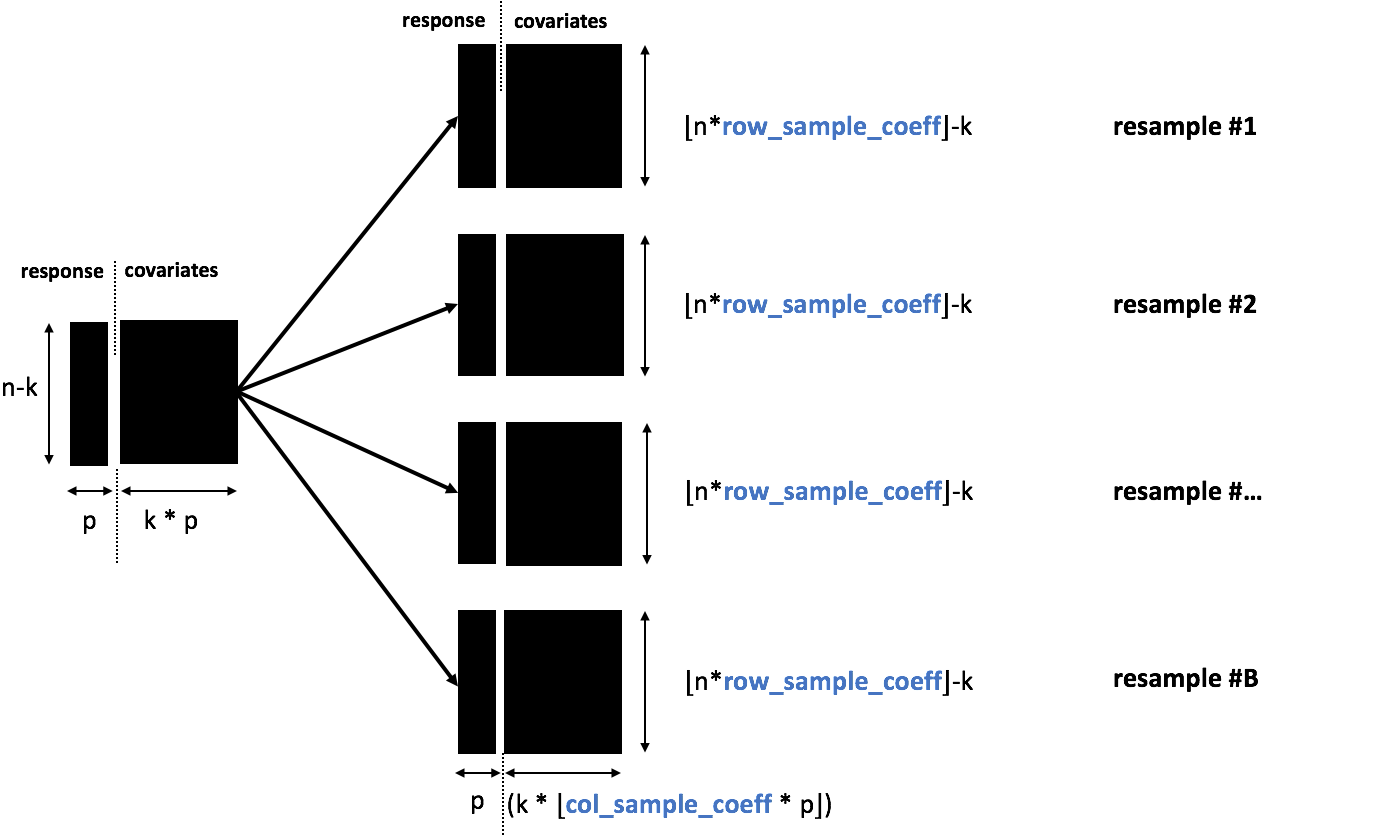
\includegraphics[width=10.5cm]{gfx/chapter-rvfl-ensembles/bootstrap_resampling.png}
\caption{Construction of $B$ bootstrap resamples by using the initial data}
\label{bootstrap_resampling_plot}
\end{figure}

\newpage

\subsection{Boosting}
\label{sec:rvflboosting}

The boosting approach adopted here, is described in Hothorn et al. (2010) and implemented in \proglang{R} package \code{mboost}. The general idea of the algorithm is to fit the in-sample residuals with base-learners, iteratively and slowly, but to stop learning before the out-of-sample error starts to worsen. With the response being $y$ and the covariates stored in  $\textbf{x}$, we are interested in constructing a regression function $\hat{f}$, so that: 
$$
\hat{f}(\textbf{x}) = \sum_{j=1}^B \nu \hat{f}_j(\textbf{x}) 
$$
$B$ is the number of boosting iterations, $\nu$ is a learning rate parameter preventing the base learners from fitting the residuals too quickly, and  $\hat{f}_j$, $j \in \left \lbrace 1, \ldots, B \right \rbrace$ are the base learners, which are obtained as: 
$$
\left(\hat{f}_1, \ldots,  \hat{f}_p\right) = argmin_{f_1, \ldots, f_p}  \rho \left( y, \sum_j \nu f_j\left( \textbf{x} \right) \right) 
$$

In this expression, $\rho$ is a loss function to be minimized (for example $x \mapsto x^2$, or $x \mapsto |x|$). And in the case of multivariate time series, we are doing multitask learning. Each series (their most contemporaneous observations) share the same set of predictors (their lagged observations) as in the RVFL model described in section \ref{sec:basemodeldesc}, but without regularization of the regression models' parameters. This model is a different version of the Stochastic Configuration Network model from (cite Wang et al. (2017)). They do not include the \textit{direct link} (linear part of the RVFL) but only the transformed predictors $\Phi(\bfX)^{(l)}= g\left(\sum_{j = 1}^p W^{(j, l)} X_i^{(j)}\right)$, and show that under certain specific conditions, the model verifies an universal approximator property. 

The same number of boosting iterations and the same learning rate are used for all the observed time series. It would be possible to consider different numbers of iterations and different learning rates for each time series, but in this situation there would be as much as parameters as time series, and the regularization parameters would be trickier to optimize. 

\subsection{Stacking}
\label{sec:rvflstacking}

Stacked generalization or stacking, was introduced (cite Wolpert (1992)). It is also presented in (Breiman (2001)) for regression models. The idea behind this procedure is to construct new predictors for the training data set, by using diverse predictions of multiple models, which are combined by a meta-learner model. A simple example of 2-fold stacking applied to regression is described hereafter. It is possible to imagine examples with more stacked layers:

\begin{itemize}
\item Divide the original training data set $\textbf{X} \in \RR^{n \times p}$, into two parts: \code{part1} and \code{part2}, each with $n/2$ rows
\item Train a base learner model on \code{part1} and obtain $n/2$ predictions on \code{part2}.
\item Train the same base learner model on \code{part2} and obtain $n/2$ predictions on \code{part1}.
\item Train a  meta-learner model on the new data set \code{part3}, consisting in the the original predictors, plus the predictors constructed by applying the base learner model on \code{part1} and \code{part2}.
\end{itemize}
\medskip

Typically, in this procedure, various types of base learners are used, to increate the diversity of new predictors. Since we are using time series data here, which inherently exhibit a serial dependence between the observations, we have to adapt the procedure described previously. In the case of a 2-fold stacking again, we divide the original training data set  $\textbf{X} \in \RR^{n \times p}$ (with $p$ time series observed at $n$ dates) into two parts: \code{part1} and \code{part2}; each consisting of $n/2$ rows. \code{part1} contains the most ancient observations and \code{part2}, the most recent observations of the time series contained in $\textbf{X}$. Also, we use multiple resamples of the base learner, as follows (this procedure is also described in figure \ref{rvfl_stacking_plot}):

\begin{itemize}
\item Train $B$ resampled RVFL models on \code{part1}, using a random subset of \code{part1} in each resampling iteration. Obtain $B$ sets of predictions ($B \times p$ new predictors) with these models, over the whole horizon  of \code{part2}.
\item Create a new enriched data set \code{part3}, containing the observed time series from \code{part2}, and the $B \times p$ additional series predicted from \code{part1} on \code{part2}.
\item Use a meta-learning model to obtain predictions on the new, enriched dataset, \code{part3}.
\end{itemize}

For the latter point, we consider a few meta-learner models that have been used in the past in the literature (cite Breiman's Stacked Regressions). In general, the idea is that a relatively simple meta-learner will achieve a good performance. We use the following models for this purpose:
\begin{itemize}
\item Linear \textbf{least squares regression} model
\item Linear least squares regression model \textbf{with positive coefficients} (cite Lawson CL, Hanson RJ (1974)) and Lawson CL, Hanson RJ (1995), as used in (cite Breiman (2001))
\item \textbf{Ridge regression} (cite Hoerl et Kennard 1970)
\end{itemize}

These selected meta-learners are trained on \code{part3}, with the most contemporaneous observations of the series as responses, and their respective lags as predictors. Some numerical examples on the application of stacking to RVFL base learners can be found in section \ref{sec:numericalexamples}

\begin{figure}[!htb]
\centering
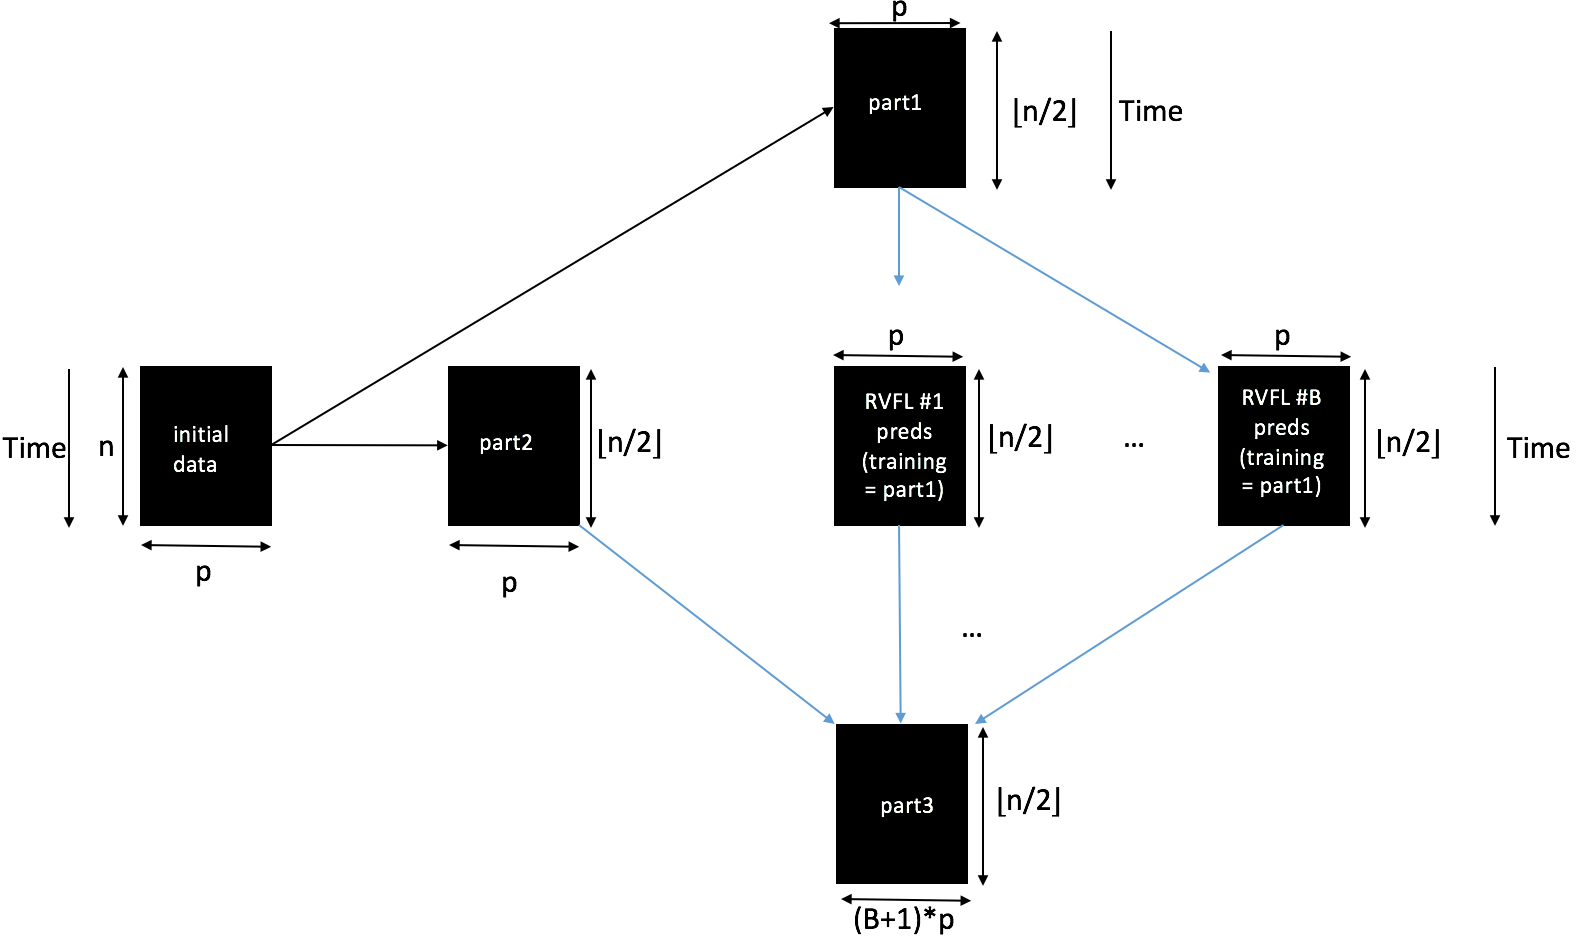
\includegraphics[width=13cm]{gfx/chapter-rvfl-ensembles/rvfl_stacking.png}
\caption{Construction of the enriched/stacked dataset}
\label{rvfl_stacking_plot}
\end{figure}


\section{Numerical examples}
\label{sec:numericalexamples}

For the numerical examples, we obtain forecast of the Treasury Bill rates among other macroeconomic variables, in a \textit{data-rich} environment. We use data from (cite Greene (20something)). Four of the time series are considered: the Treasury Bill rates, the real consumption, the consumer price index, and the real expenditure. They are all observed on a quaterly basis. 

We annualize the last three time series, but keep the Treasury Bill rates unchanged. So that, the four time series are nearly on the same scale.

The out-of-sample Root Mean Squared Error (RMSE) is used as a measure of performance of the different implemented models.

\subsection{Descriptive statistics}

Figure \ref{all_series_plot} presents the resulting time series' data obtained after the few transformations described in the previous paragraph. Table \ref{tab:summary_four_ts} contains a summary of these data, where we can see that the four time series are now nearly expressed in the same scale.

\begin{figure}[!htb]
\centering
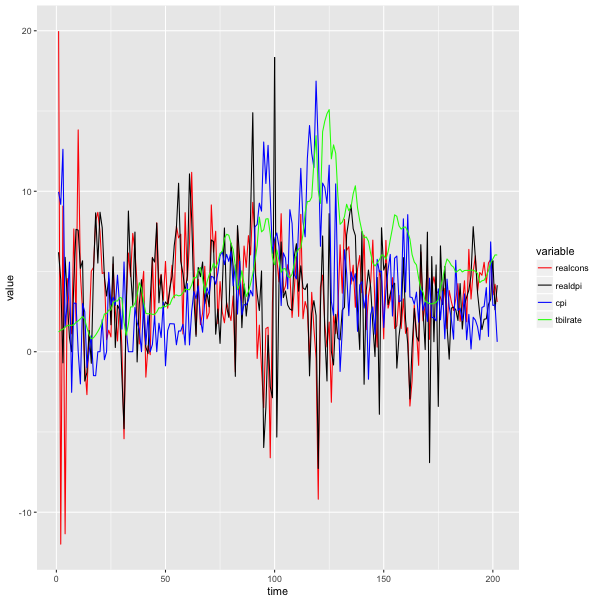
\includegraphics[width=10cm]{gfx/chapter-rvfl-ensembles/all_series.png}
\caption{Treasury Bills rates and transformed Real consumption, Real disposable income, and  Inflation data from (cite Greene et. al (2007)) in a \textit{data-rich} environment}
\label{all_series_plot}
\end{figure}


\begin{table}[!htb]
\begin{center}
% table caption is above the table
\caption{Summary statistics for the four transformed time series: Treasury Bills and transformed Real consumption, Real disposable income, and  Inflation data from (cite Greene et. al (2007))}
\label{tab:summary_four_ts}       % Give a unique label
% For LaTeX tables use
\begin{tabular}{llllllll}
\hline\noalign{\smallskip}
Series & Min & 1st Qrt  & Median  & Mean & 3rd Qrt  & Max & Std. Dev.\\
\noalign{\smallskip}\hline\noalign{\smallskip}
  Real consumption  & -11.990 & 1.814 & 3.637 & \textbf{3.513} & 5.414 & 19.978 & \textbf{3.546}\\
  Real disposable income  & -7.275 & 1.613 & 3.390 & \textbf{3.423} & 5.518 & 18.358 & \textbf{3.486}\\
  Inflation & -2.530  & 1.755 & 3.135 & \textbf{3.936} & 5.593 & 16.864 & \textbf{3.407}\\
  Treasury Bills rates & 0.810  & 3.138 & 5.050 & \textbf{5.270} & 6.715 & 15.090 & \textbf{2.829} \\
\noalign{\smallskip}\hline
\end{tabular}
\end{center}
\end{table}


\begin{table}
\begin{center}
% table caption is above the table
\caption{\textbf{Box-Pierce test for the independence} in the time series observations}
\label{tab:boxpierce}       % Give a unique label
% For LaTeX tables use
\begin{tabular}{llllll}
\hline\noalign{\smallskip}
Series &  \code{X-squared} & \code{p-value}  \\
\noalign{\smallskip}\hline\noalign{\smallskip}
  Real consumption & 0.0133 & \textbf{0.9082}  \\
  Real disposable income & 1.3912 & \textbf{0.2382} \\
  Inflation & 86.428 &  2.2e-16 \\
  Treasury Bills rates & 186.35 & 2.2e-16 \\
\noalign{\smallskip}\hline
\end{tabular}
\end{center}
\end{table}

\begin{figure}[!htb]
\centering
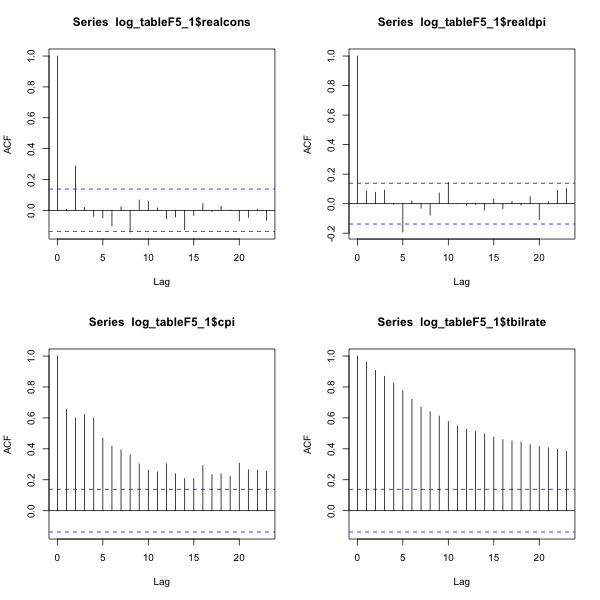
\includegraphics[width=12cm]{gfx/chapter-rvfl-ensembles/acf.png}
\caption{Autocorrelation function for the four times series: Treasury Bills rates, Real consumption, Real disposable income, Inflation}
\label{acf}
\end{figure}

\newpage

The Box-Pierce tests results presented in table \ref{tab:boxpierce}, and the autocorrelation functions presented in \ref{acf}, show that the two time series for Real consumption and Real disposable income could be considered as stationary after the transformations. Whereas for the Treasury Bills rates and Inflation, there is still a non-negligible autocorrelation within the series. 

\medskip

Another interesting information is given by figure \ref{corrplot}. We observe that the distribution of the data for inflation and Treasury Bills rates is skewed, when compared to the data for Real consumption and Real disposable income. 

\medskip

Also, based on the correlations displayed in figure \ref{corrplot}, the Real consumption is globally  decreasing when the Treasury Bills rates and the inflation are increasing. But when the Real disposable income increases, the Real consumption increases as well. 

\begin{figure}[!htb]
\centering
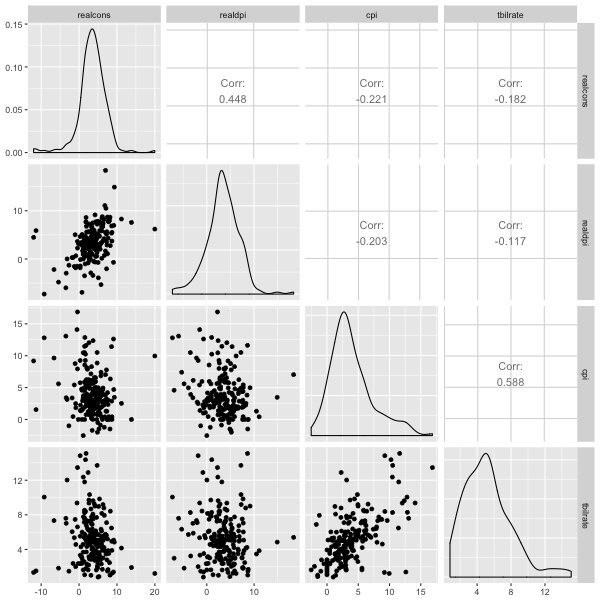
\includegraphics[width=14cm]{gfx/chapter-rvfl-ensembles/scatterplot.png}
\caption{Correlation plot for the four times series: Treasury Bills rates, Real consumption, Real disposable income, Inflation}
\label{corrplot}
\end{figure}

%\newpage

In sections \ref{bagging_example} and \ref{stacking_example}, we apply the bagging and stacking procedures described in sections \ref{sec:rvflbagging} and \ref{sec:rvflstacking} to the dataset we have just described. 


A rolling forecasting cross-validation method (see \cite{bergmeir2015note} and figure \ref{rolling_cv}). At the beginning of the procedure, the training set contains $24$ points ($4$ years), and the test set contains $4$ points ($1$ year) and $8$ points ($2$ years). The training set is then advanced of one point forward (rolled), and the procedure is repeated until no more data for the training set are found.  

\begin{figure}[!htb]
\centering
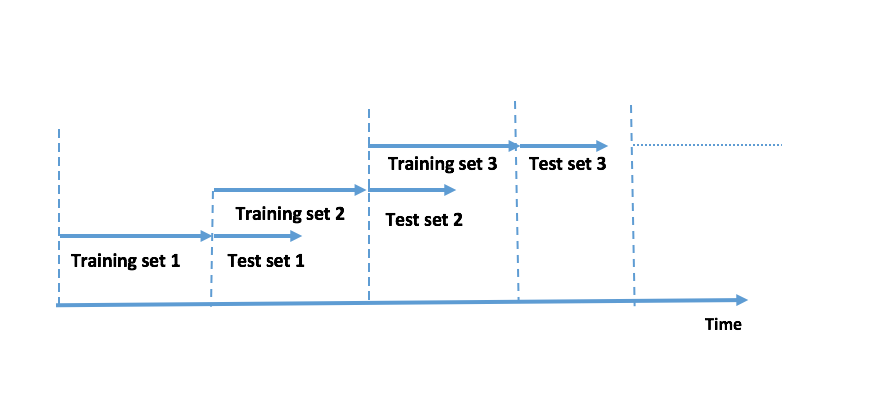
\includegraphics[width=14cm]{gfx/chapter-rvfl-ensembles/rolling_cv.png}
\caption{Training and testing sets in rolling forecasting cross-validation}
\label{rolling_cv}
\end{figure}

As we said at the beginning of section \ref{sec:numericalexamples}, we use the Root Mean Squared Error (RMSE) as a measure of the out-of-sample error. All the benchmarks are made on what is defined as \code{part3} in section \ref{sec:rvflstacking}, in order to have a similar perimeter for bagging and stacking. The results obtained by the ensemble learners are compared to those obtained by the base RVFL model, which are presented here: 

For the bagging example, we use $B = 100$ resamples of the data, and calculate the average out-of-sample RMSE obtained by the ensemble model on all the testing sets (see figure \ref{rolling_cv}). The dataset used, is the one defined as \code{part3} in section \ref{sec:rvflstacking}.  

For the boosting example, we use $B = 10$ boosting iterations of the least squares regression model from formula ~\ref{eq:rvflequation}. The tuning parameters are the learning rate of the boosting algorithm denoted as $\nu$, the number of nodes in the hidden layer for the base-learner \code{nb\underline{  }hidden}, the fraction of the initial time series considered as predictors \code{col\underline{  }sample}, the number of lags. 

For the stacking example, The dataset used, is also the one defined as \code{part3} in section \ref{sec:rvflstacking}. The tuning parameters are the number of boostrap resamples, $B$, and the hyperparameter of the ridge regression model is the regularization parameter. 

\subsection{Summary of results}
\label{results_summary}

A summary of the out-of-sample RMSE is presented in figure \ref{boxplot_perfs} in a logarithmic scale, for all the methods that we described and tested in the previous sections. The numerical values corresponding to these boxplots can be found in appendix \ref{boxplot_summary}, in their original scale. 

The base RVFL model is denoted as \code{ridge2}. \code{bagging}, \code{stack\underline{  }ridge}, \code{stack\underline{  }lm}, \code{stack\underline{  }nnls}, and \code{glmboost} respectively denote the bootstrap aggregating method from section \ref{sec:rvflbagging}, stacking with ridge regression, with ordinary least squares, least squares regression with positive coefficients from section \ref{sec:rvflstacking}, and boosting from section \ref{sec:rvflboosting}. We also added an unrestricted Vector AutoRegression (VAR) model to the benchmarks, denoted as \code{VAR}, which mostly helps us in assessing if the other models' implementation/predictions are not off track.  

\begin{figure}[!htb]
\centering
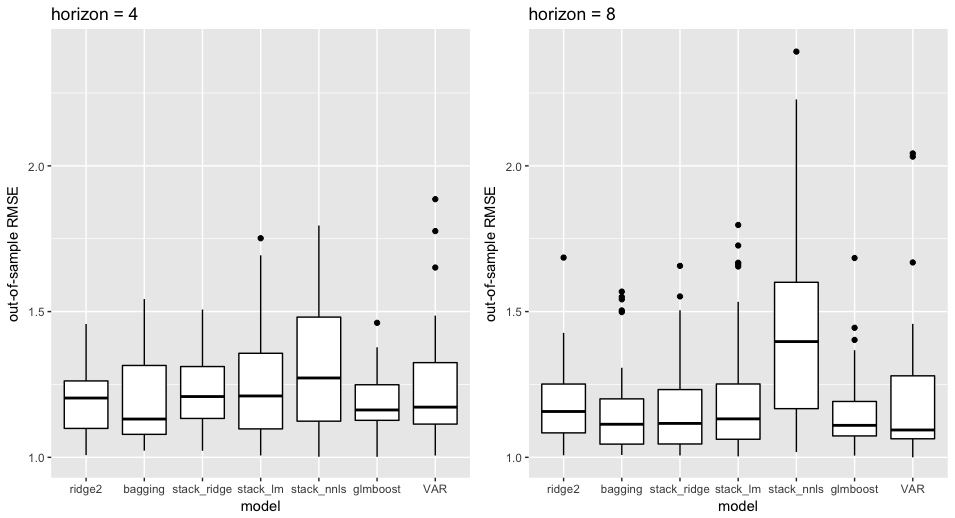
\includegraphics[width=14cm]{gfx/chapter-rvfl-ensembles/boxplot_perfs.png}
\caption{Out-of-sample RMSE distribution for the different tested models}
\label{boxplot_perfs}
\end{figure}

Bagging is performing the best on average (cf. appendix \ref{boxplot_perfs} for details) on both horizons, 4-steps ahead and 8-steps ahead, and is followed by boosting. The stacking algorithm works best with the ridge regression model taken as a meta-learner, but is failing with the other meta learners (ordinary least squares and least squares regression with positive coefficients). Overall, the boosting algorithm is also very robust, and displays the lowest standard deviation of all the models tested. 

The \textit{best} hyperparameters obtained for each algorithm are presented below, for the different horizons of projection. The best hyperparameter found for stacking with ordinary least squares, with a constraint on the regression parameters or not, is the number of lags equal to $1$ and $B = 1$. 

\textbf{For horizon = 4}

\begin{table}[!htb]
\begin{center}
% table caption is above the table
\caption{\textit{Best} hyperparameters for the base RVFL}
\label{tab:bestparamsrvfl}       % Give a unique label
% For LaTeX tables use
\begin{tabular}{lllllll}
\hline\noalign{\smallskip}
Method & lags & nodes & $\lambda_1$ & $\lambda_2$ &   &   \\
\noalign{\smallskip}\hline\noalign{\smallskip}
  \textbf{RVFL} & 3 & 100 & 10000 & 100 &  &  \\
\noalign{\smallskip}\hline
\end{tabular}
\end{center}
\end{table}

\begin{table}[!htb]
\begin{center}
% table caption is above the table
\caption{\textit{Best} hyperparameters for the bagging of RVFLs}
\label{tab:bestparamsbagrvfl}       % Give a unique label
% For LaTeX tables use
\begin{tabular}{llllllll}
\hline\noalign{\smallskip}
Method & lags & nodes & $\lambda_1$ & $\lambda_2$ & B  &  col. sample  & row. sample\\
\noalign{\smallskip}\hline\noalign{\smallskip}
  \textbf{Bagging} & 1 & 1 & 21.54435 & 21.54435 & 100 & 0.9 & 0.9\\
\noalign{\smallskip}\hline
\end{tabular}
\end{center}
\end{table}

\begin{table}[!htb]
\begin{center}
% table caption is above the table
\caption{\textit{Best} hyperparameters for the stacking with ridge regression}
\label{tab:bestparamsbagrvfl}       % Give a unique label
% For LaTeX tables use
\begin{tabular}{llllllll}
\hline\noalign{\smallskip}
Method & lags & $\lambda$ & $B$ & col. sample  &  row. sample  \\
\noalign{\smallskip}\hline\noalign{\smallskip}
  \textbf{Stacking (ridge)} & 3 & 21.54435 &  1 & 0.9 & 0.8   \\
\noalign{\smallskip}\hline
\end{tabular}
\end{center}
\end{table}

\begin{table}[!htb]
\begin{center}
% table caption is above the table
\caption{\textit{Best} hyperparameters for the boosting algorithm}
\label{tab:bestparamsbagrvfl}       % Give a unique label
% For LaTeX tables use
\begin{tabular}{llllllll}
\hline\noalign{\smallskip}
Method & lags & nodes & $\nu$ & $B$ & col. sample  &  & \\
\noalign{\smallskip}\hline\noalign{\smallskip}
  \textbf{Boosting} & 3 & 1 & $0.2020798$ & 10 & 1 & & \\
\noalign{\smallskip}\hline
\end{tabular}
\end{center}
\end{table}

\begin{table}[!htb]
\begin{center}
% table caption is above the table
\caption{\textit{Best} hyperparameters for the VAR}
\label{tab:bestparamsvar}       % Give a unique label
% For LaTeX tables use
\begin{tabular}{llllllll}
\hline\noalign{\smallskip}
Method & lags & type of regressor &  &  &  &  & \\
\noalign{\smallskip}\hline\noalign{\smallskip}
  \textbf{VAR} & 1 & const &  & &  & & \\
\noalign{\smallskip}\hline
\end{tabular}
\end{center}
\end{table}


\textbf{For horizon = 8}

\begin{table}[!htb]
\begin{center}
% table caption is above the table
\caption{\textit{Best} hyperparameters for the base RVFL}
\label{tab:bestparamsrvfl}       % Give a unique label
% For LaTeX tables use
\begin{tabular}{lllllll}
\hline\noalign{\smallskip}
Method & lags & nodes & $\lambda_1$ & $\lambda_2$ &   &   \\
\noalign{\smallskip}\hline\noalign{\smallskip}
  \textbf{RVFL} & 3 & 2 & 21.54435 & 10000 &  &  \\
\noalign{\smallskip}\hline
\end{tabular}
\end{center}
\end{table}

\begin{table}[!htb]
\begin{center}
% table caption is above the table
\caption{\textit{Best} hyperparameters for the bagging of RVFLs}
\label{tab:bestparamsbagrvfl}       % Give a unique label
% For LaTeX tables use
\begin{tabular}{llllllll}
\hline\noalign{\smallskip}
Method & lags & nodes & $\lambda_1$ & $\lambda_2$ & B  &  col. sample  & row. sample\\
\noalign{\smallskip}\hline\noalign{\smallskip}
  \textbf{Bagging} & 1 & 1 & 21.54435 & 21.54435 & 100 & 0.9 & 0.9\\
\noalign{\smallskip}\hline
\end{tabular}
\end{center}
\end{table}

\begin{table}[!htb]
\begin{center}
% table caption is above the table
\caption{\textit{Best} hyperparameters for the stacking with ridge regression}
\label{tab:bestparamsbagrvfl}       % Give a unique label
% For LaTeX tables use
\begin{tabular}{llllllll}
\hline\noalign{\smallskip}
Method & lags & $\lambda$ & $B$ & col. sample  &  row. sample  \\
\noalign{\smallskip}\hline\noalign{\smallskip}
  \textbf{Stacking (ridge)} & 3 & 21.54435 &  1 & 0.9 & 0.9   \\
\noalign{\smallskip}\hline
\end{tabular}
\end{center}
\end{table}

\begin{table}[!htb]
\begin{center}
% table caption is above the table
\caption{\textit{Best} hyperparameters for the boosting algorithm}
\label{tab:bestparamsbagrvfl}       % Give a unique label
% For LaTeX tables use
\begin{tabular}{llllllll}
\hline\noalign{\smallskip}
Method & lags & nodes & $\nu$ & $B$ & col. sample  &  & \\
\noalign{\smallskip}\hline\noalign{\smallskip}
  \textbf{Boosting} & 3 & 1 & $0.175$ & 10 & 1 & & \\
\noalign{\smallskip}\hline
\end{tabular}
\end{center}
\end{table}

\begin{table}[!htb]
\begin{center}
% table caption is above the table
\caption{\textit{Best} hyperparameters for the VAR}
\label{tab:bestparamsvar}       % Give a unique label
% For LaTeX tables use
\begin{tabular}{llllllll}
\hline\noalign{\smallskip}
Method & lags & type of regressor &  &  &  &  & \\
\noalign{\smallskip}\hline\noalign{\smallskip}
  \textbf{VAR} & 1 & none &  & &  & & \\
\noalign{\smallskip}\hline
\end{tabular}
\end{center}
\end{table}

\newpage

Below, in figure \ref{oos_rmse_over_time}, we can observe how the different methods perform through time. We observe that the models' errors are highly correlated, which is reassuring concerning their implementation. 

\begin{figure}[!htb]
\centering
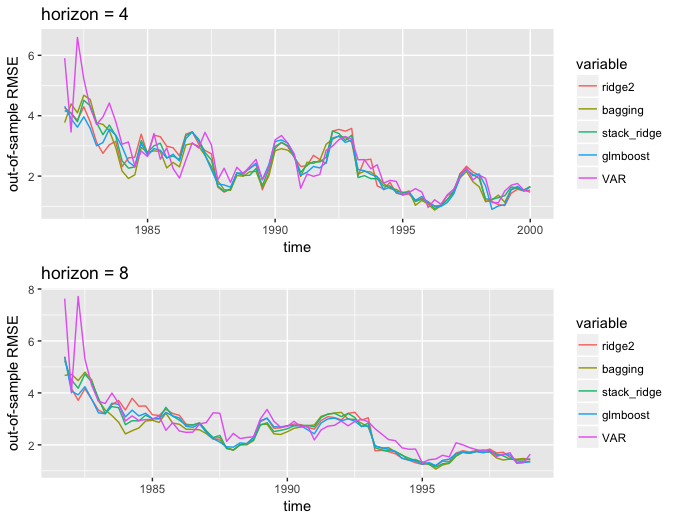
\includegraphics[width=14cm]{gfx/chapter-rvfl-ensembles/oos_rmse_over_time.png}
\caption{Out-of-sample RMSE over time for the different tested models + VAR}
\label{oos_rmse_over_time}
\end{figure}

The details of the correlations between these errors can be found in appendix \ref{oos_errors_cor}. The VAR model generally exhibits a higher variance than the other models (excluding stacking with \code{stack\underline{  }lm} and \code{stack\underline{  }nnls}), but is still able to perform better than them at times (due to the high variance).    

\newpage

\section{Appendix}

\subsection{Out-of-sample errors summary}
\label{boxplot_summary}

\textbf{horizon = 4}

\begin{itemize}

\item Min., 1st Qu., Median, Mean, 3rd Qu., Max

\begin{verbatim}
 ridge2           bagging          stack_ridge      stack_lm         
 Min.   :0.9995   Min.   :0.8746   Min.   :0.9291   Min.   :0.9784   
 1st Qu.:1.5529   1st Qu.:1.5908   1st Qu.:1.6426   1st Qu.:1.7379   
 Median :2.3605   Median :2.1484   Median :2.2407   Median :2.1715      
 Mean   :2.3763   Mean   :2.3034   Mean   :2.3676   Mean   :2.5058      
 3rd Qu.:3.0261   3rd Qu.:2.8957   3rd Qu.:3.0690   3rd Qu.:3.0031      
 Max.   :4.2952   Max.   :4.6781   Max.   :4.5133   Max.   :5.7641
 
 stack_nnls           glmboost          VAR
 Min.   :0.9874       Min.   :0.8996    Min.   :1.041 
 1st Qu.:1.7273       1st Qu.:1.6477    1st Qu.:1.680
 Median :2.2839       Median :2.2443    Median :2.146
 Mean   :2.5115       Mean   :2.3261    Mean   :2.498
 3rd Qu.:3.0494       3rd Qu.:3.0648    3rd Qu.:3.070
 Max.   :6.0210       Max.   :4.3121    Max.   :6.068
\end{verbatim}

\item Standard deviation

\begin{verbatim}
   ridge2   bagging stack_ridge    stack_lm  stack_nnls    glmboost   VAR
0.8804324 0.8881329   0.8870853   1.0549136   1.0889430   0.8238531   1.0511201
\end{verbatim}

\end{itemize}

\textbf{horizon = 8}

\begin{itemize}

\item Min., 1st Qu., Median, Mean, 3rd Qu., Max

\begin{verbatim}
  ridge2         bagging       stack_ridge       stack_lm               
 Min.   :1.192   Min.   :1.066   Min.   :1.143   Min.   :1.253      
 1st Qu.:1.740   1st Qu.:1.717   1st Qu.:1.754   1st Qu.:1.813      
 Median :2.663   Median :2.467   Median :2.656   Median :2.694      
 Mean   :2.529   Mean   :2.440   Mean   :2.509   Mean   :2.676      
 3rd Qu.:3.154   3rd Qu.:2.868   3rd Qu.:3.041   3rd Qu.:3.065      
 Max.   :5.394   Max.   :4.800   Max.   :5.243   Max.   :6.032      
 
 stack_nnls           glmboost          VAR
 Min.   : 1.164       Min.   :1.203     Min.   :1.289
 1st Qu.: 2.056       1st Qu.:1.718     1st Qu.:1.920
 Median : 2.775       Median :2.683     Median :2.648 
 Mean   : 3.331       Mean   :2.478     Mean   :2.696 
 3rd Qu.: 4.069       3rd Qu.:3.024     3rd Qu.:2.964
 Max.   :10.935       Max.   :5.387     Max.   :7.711
\end{verbatim}

\item Standard deviation

\begin{verbatim}
   ridge2     bagging stack_ridge    stack_lm  stack_nnls    glmboost         VAR
0.8955453   0.8883188   0.9093582   1.0406195   1.8865643   0.8547240   1.1482777 
\end{verbatim}

\end{itemize}

\subsection{Correlation of out-of-sample errors}
\label{oos_errors_cor}

\textbf{horizon = 4}

\begin{verbatim}
            ridge2   bagging      stack_ridge  glmboost       VAR
ridge2      1.0000000 0.9350414   0.9658978    0.9627834      0.8422500
bagging     0.9350414 1.0000000   0.9796091    0.9388819      0.8746823
stack_ridge 0.9658978 0.9796091   1.0000000    0.9731609      0.8758017
glmboost    0.9627834 0.9388819   0.9731609    1.0000000      0.8840573
VAR         0.8422500 0.8746823   0.8758017    0.8840573      1.0000000
\end{verbatim}

\textbf{horizon = 8}

\begin{verbatim}
                ridge2  bagging stack_ridge  glmboost       VAR
ridge2      1.0000000 0.9280983   0.9693424 0.9909838 0.8185879
bagging     0.9280983 1.0000000   0.9855720 0.9481774 0.8522099
stack_ridge 0.9693424 0.9855720   1.0000000 0.9804522 0.8561227
glmboost    0.9909838 0.9481774   0.9804522 1.0000000 0.8622763
VAR         0.8185879 0.8522099   0.8561227 0.8622763 1.0000000
\end{verbatim}